\documentclass[11pt,a4paper]{report}

\usepackage[utf8]{inputenc}
\usepackage{titling}
\usepackage[german]{babel}
\usepackage[T1]{fontenc}
\usepackage{amsmath}
\usepackage{amsfonts}
\usepackage{amssymb}
\usepackage[left=3cm,right=2cm,top=2.5cm,bottom=2cm]{geometry}
\usepackage{graphicx}
\usepackage{fancyhdr}
\usepackage{color}
\usepackage[
colorlinks=true,
urlcolor=blue,
linkcolor=black
]{hyperref}
\pagestyle{fancy}

\lhead{Sina Opitz}
\chead{ak18b}
\rhead{13.01.2019}

\lfoot{}
\cfoot{\thepage}
\rfoot{}

\renewcommand{\headrulewidth}{0.4pt}
\renewcommand{\footrulewidth}{0.4pt}

\begin{document}
	\begin{titlepage}
		
		\pretitle{
			\vskip -3em
			\begin{figure}[h]
				\begin{center}
					
\includegraphics[scale=0.55]{Logo.png}
				\end{center}
			\end{figure}
			\begin{center}
				\vskip -2em
				\large{Wintersemester 2018/19\\Softwaretechnikpraktikum} \vskip 9em
				\rule{5in}{0.4pt}\par \vskip 0.5em
			}
			\posttitle{\par\rule{5in}{0.4pt} \vskip 4em
				\Large Gruppe: ak18b \vskip 1.5em
				\normalsize Betreuer: Benjamin Lucas Friedland, Michael Fritz\vskip 1em
				\normalsize Gruppenmitglieder: Alexander Zwisler, Leon Kamuf, Leon Rudolph, Maurice Eisenblätter, Maximilian Gläfcke, Robin Seidel, Sina Opitz, Steve Woywod
		\end{center}}
		
		\title{\textbf{\Huge App zur Inventarisierung von Unternehmenswerten}\vskip 0.5em \huge Entwurfsbeschreibung}
		\date{}
		\maketitle
	\end{titlepage}
	\setcounter{secnumdepth}{4}
	\setcounter{tocdepth}{4}
	\tableofcontents
	\thispagestyle{empty}
	\newpage
	\setcounter{page}{1}
	\renewcommand\thesection{\arabic{section}}
	
	\section{Allgemeine Informationen}
	\subsection{Einführung}
Herzlich Willkommen!
\\~\\
Dieses Handbuch hilft Ihnen die Inventarisierungsapp optimal zu nutzen.\\
Wir wünschen Ihnen viel Freude bei der Nutzung!\\
Optimiert wurde die Web-App für Google Chrome.
\\~\\
Änderungen vorbehalten\\
Version 1/11.03.19
	\subsection{Ihre Vorteile}
	\begin{itemize}
		\item intuitive Benutzeroberfläche
		\item für jedes Unternehmen geeignet
		\item vollständige digitale Inventarisierung
		\item übersichtliche Darstellung aller Gegenstände
		\item Erstellen von Benutzerrollen zur Sicherung aller Gegenstände
		\item Gruppieren der Gegenstände nach Typen
	\end{itemize}
	\section{Erste Schritte}
	\textbf{Die App läuft vollständig im Browser. Es ist also keine Installation auf Ihrem Rechner nötig!}\\
	Empfohlener Browser: Google Chrome
	
	\begin{itemize}
		\item Rufen Sie im Browser die App auf
		\item Loggen Sie sich mit Ihrem Benutzernamen und Passwort an
	\end{itemize}
	
	\section{Verwenden der Inventarisierungsapp}
	\subsection{Einen Objekttypen hinzufügen}
	
	\begin{enumerate}
		\item Klicken Sie auf \glqq{}Objekttypen\grqq{}
		\item Klicken Sie auf \texttt{+} neben der Suchleiste
	\end{enumerate}\\

	\begin{minipage}{0.4\linewidth}
	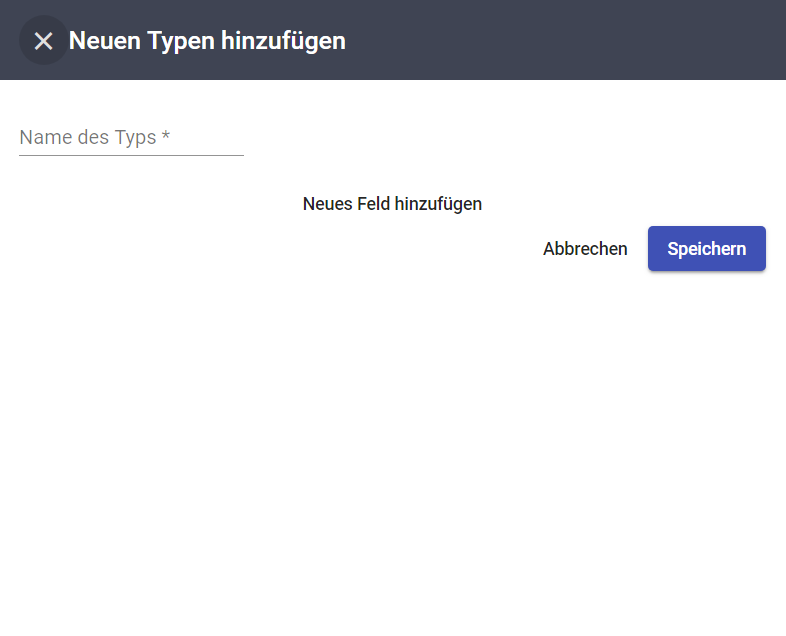
\includegraphics[scale=0.55]{Objekttyp.png}
	\end{minipage}
	\hfill
	\begin{minipage}{0.4\linewidth}
	\begin{enumerate}[3]
		\item Wählen Sie einen Namen für Ihren Objekttypen (1)
		\item Fügen Sie beliebig viele Felder hinzu (2)
	\end{enumerate}
	\end{minipage}\\

	\begin{minipage}{0.4\linewidth}
	\includegraphics[scale=0.55]{Objekttypfeld.png}
	\end{minipage}
	\hfill
	\begin{minipage}{0.4\linewidth}
	\begin{enumerate}[5]
		\item Wählen Sie einen Datentypen (1)
		\item Wählen Sie einen Namen für das Feld (2)
		\item Entscheiden Sie, ob das Feld ein Pflichtfeld sein soll (3)
		\item Entscheiden Sie, ob das Feld einzigartig sein soll (4)
		\item Klicken Sie auf Speichern
	\end{enumerate}
	\end{minipage}\\

	\subsection{Einen Objekttypen bearbeiten oder löschen}

	\begin{enumerate}
		\item Klicken Sie auf \glqq{}Objekttypen\grqq{}
		\item Klicken Sie auf den Objekttypen, den Sie bearbeiten oder löschen wollen
	\end{enumerate}\\

	\begin{minipage}{0.4\linewidth}
	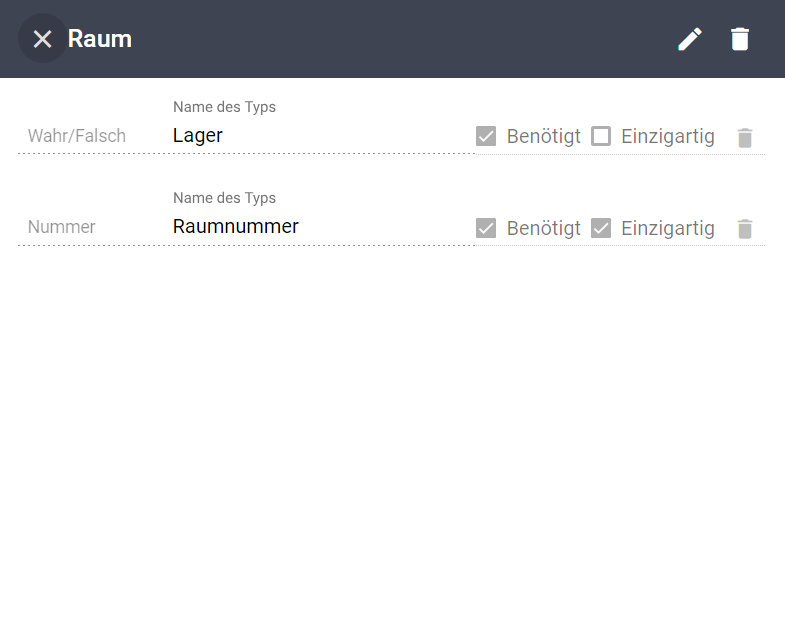
\includegraphics[scale=0.55]{Objekttypedit.png}
	\end{minipage}
	\hfill
	\begin{minipage}{0.4\linewidth}
	\begin{enumerate}[3]
		\item Wählen Sie (1) aus, um die Objekttypen zu bearbeiten
		\item Wählen Sie (2) aus, um alle Objekttypen zu löschen\\
		ACHTUNG: Löschen der Objekttypen löscht auch deren Inhalte
	\end{enumerate}
	\end{minipage}\\

	\begin{minipage}{0.4\linewidth}
	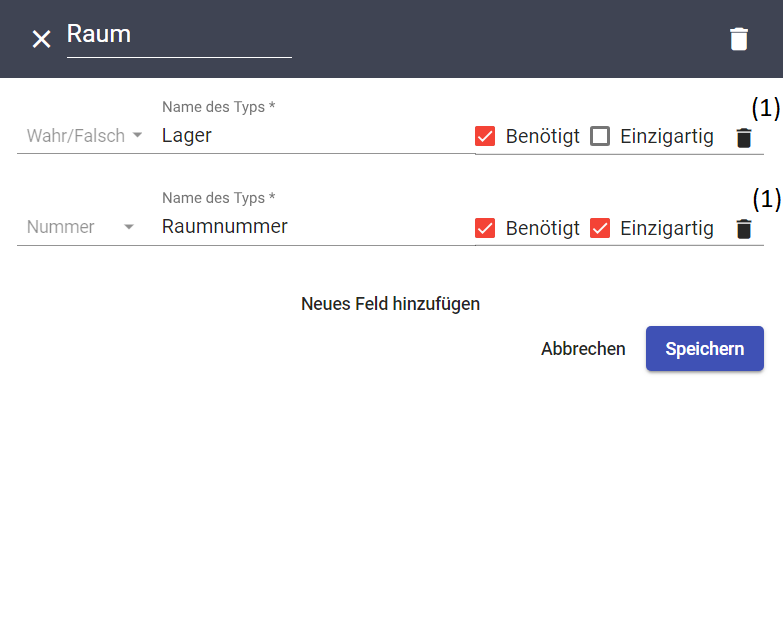
\includegraphics[scale=0.55]{Objekttypedit2.png}
	\end{minipage}
	\hfill
	\begin{minipage}{0.4\linewidth}
	\begin{enumerate}[5]
		\item Bearbeiten Sie die Felder
		\item Wählen Sie (1) aus, um den Objekttypen zu löschen\\
		ACHTUNG: Löschen des Objekttypens löscht auch den Inhalt
	\end{enumerate}
	\end{minipage}\\

	\subsection{Ein Objekt zu einem Itemtypen hinzufügen}

	\begin{enumerate}
		\item Klicken Sie auf \glqq{}Inventar\grqq{}
		\item Klicken Sie auf \texttt{+} neben der Suchleiste
	\end{enumerate}\\

	\begin{minipage}{0.4\linewidth}
	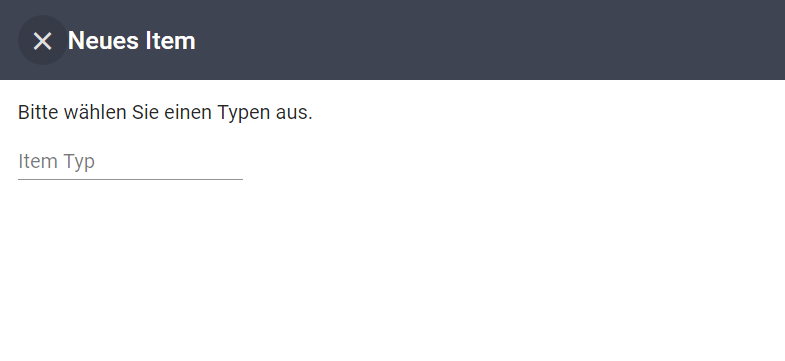
\includegraphics[scale=0.55]{Inventar.png}
	\end{minipage}
	\hfill
	\begin{minipage}{0.4\linewidth}
	\begin{enumerate}[3]
		\item Wählen Sie aus, welchem Objekttyp ein Objekt hinzugefügt werden soll (1)
		\item Füllen Sie die Felder aus (2)
		\item[] Mit * markierte Felder sind Pflichtfelder
		\item Klicken Sie auf Speichern
	\end{enumerate}
	\end{minipage}\\

	\subsection{Ein Objekt bearbeiten oder löschen}

	\begin{enumerate}
		\item Klicken Sie auf \glqq{}Inventar\grqq{}
		\item Klicken Sie auf das Objekt, das Sie bearbeiten oder löschen wollen
	\end{enumerate}\\

	\begin{minipage}{0.4\linewidth}
	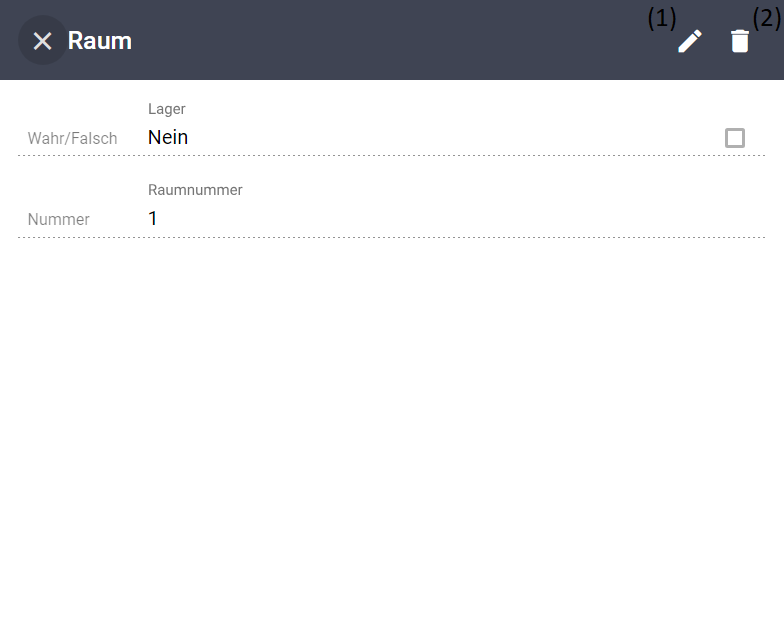
\includegraphics[scale=0.55]{ObjektInventaredit.png}
	\end{minipage}
	\hfill
	\begin{minipage}{0.4\linewidth}
	\begin{enumerate}[3]
		\item Wählen Sie (1) aus, um das Objekt zu bearbeiten
		\item Wählen Sie (2) aus, um das Objekt zu löschen
	\end{enumerate}
	\end{minipage}\\

	\subsection{Die Sprache ändern}
	\begin{enumerate}
		\item Klicken Sie auf \texttt{DE} oder \texttt{EN} (je nach Standardeinstellung) oben rechts
		\item Wählen Sie die gewünschte Sprache\\
		\texttt{en} = Englisch\\
		\texttt{de} = Deutsch
	\end{enumerate}\\

	\section{Eigene Daten bearbeiten}
	\begin{itemize}
		\item Klicken Sie auf Ihren Benutzernamen links in der Leiste
	\end{itemize}\\

	\subsection{Email-Adresse ändern}
		\begin{itemize}
		\item Wählen Sie eine neue gültige Email-Adresse
	\end{itemize}\\

	\subsection{Passwort ändern}
	\begin{enumerate}
		\item Bestätigen Sie Ihr altes Passwort
		\item Wählen Sie ein neues Passwort
		\item Bestätigen Sie das neue Passwort
	\end{enumerate}\\

	\section{Funktionen für den Admin}
	\subsection{eine Benutzerrolle hinzufügen}

	\begin{enumerate}
		\item Klicken Sie auf \glqq{}Benutzerrollen\grqq{}
		\item Klicken Sie auf \texttt{+} neben der Suchleiste
	\end{enumerate}\\

	\begin{minipage}{0.4\linewidth}
	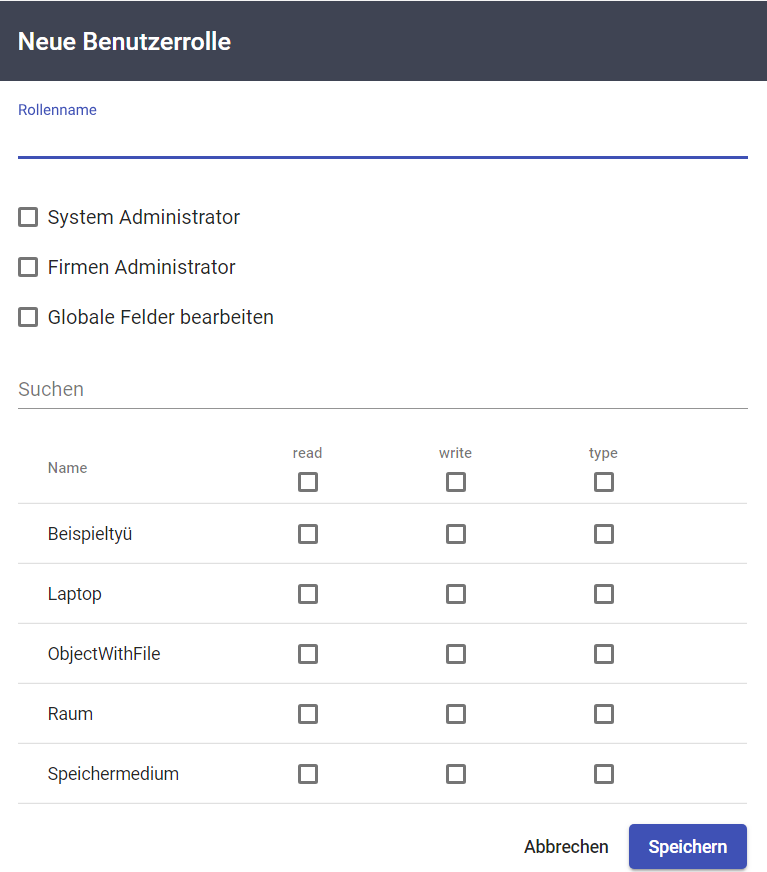
\includegraphics[scale=0.55]{Rollen.png}
	\end{minipage}
	\hfill
	\begin{minipage}{0.4\linewidth}
	\begin{enumerate}[3]
		\item Wählen Sie einen Namen für die Benutzerrolle aus
		\item Entscheiden Sie, ob die Benutzerrolle System Administrator, Firmen Administrator ist und ob sie globale Felder bearbeiten können soll\\
		System Administrator = Darf alle Objekttypen, Objekte und Benutzer aller Firmen verwalten
		Firmen Administrator = Darf alle Objekttypen, Objekte und Benutzer der Firma, die er angehört, verwalten
		\item Entscheiden Sie, welche Objekttypen die Benutzerrolle lesen (1) oder bearbeiten (2) kann
	\end{enumerate}
	\end{minipage}\\

	\subsection{eine Benutzerrolle bearbeiten}

	\begin{enumerate}
		\item Klicken Sie auf \glqq{}Benutzerrollen\grqq{}
		\item Klicken Sie auf die Benutzerrolle, die Sie bearbeiten wollen
	\end{enumerate}\\

	\begin{minipage}{0.4\linewidth}
	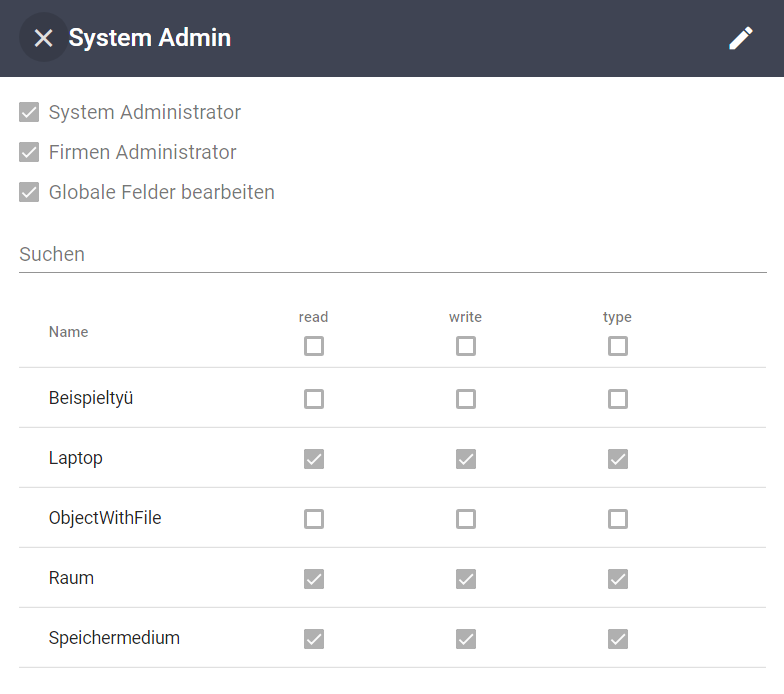
\includegraphics[scale=0.55]{Rollenedit.png}
	\end{minipage}
	\hfill
	\begin{minipage}{0.4\linewidth}
	\begin{enumerate}[3]
		\item Wählen Sie (1) aus, um die Benutzerrolle zu bearbeiten
		\item Ändern Sie die geünschten Rechte
		\item Klicken Sie auf Speichern
	\end{enumerate}
	\end{minipage}\\

	\subsection{Einen Benutzer einer Benutzerrolle hinzufügen}
	
	\begin{enumerate}
		\item Klicken Sie auf \glqq{}Benutzer\grqq{}
		\item Klicken Sie auf \texttt{+} neben der Suchleiste
	\end{enumerate}\\

	\begin{minipage}{0.4\linewidth}
	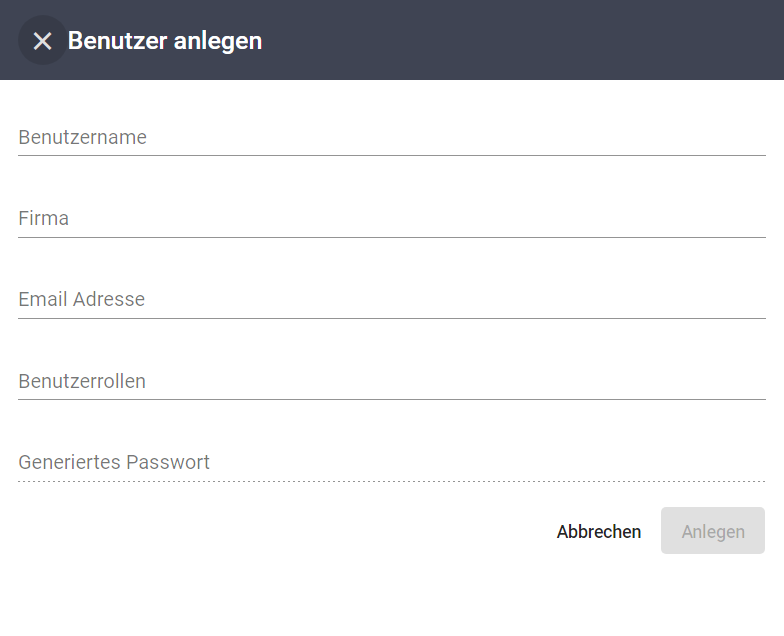
\includegraphics[scale=0.55]{Benutzer.png}
	\end{minipage}
	\hfill
	\begin{minipage}{0.4\linewidth}
	\begin{enumerate}[3]
		\item Wählen Sie einen Namen für den Benutzer aus (1)
		\item Entscheiden Sie, welcher Firmer der Benutzer angehören soll (2)
		\item Geben Sie eine gültige Email-Adresse an (3)
		\iten Entscheiden Sie, welche Benutzerrollen der Benutzer haben soll(4)
		\item Klicken Sie auf Speichern
	\end{enumerate}
	\end{minipage}\\

	\subsection{Einen Benutzer bearbeiten}

		\begin{enumerate}
		\item Klicken Sie auf \glqq{}Benutzer\grqq{}
		\item Klicken Sie auf den Benutzer, den Sie bearbeiten wollen
	\end{enumerate}\\

	\begin{minipage}{0.4\linewidth}
	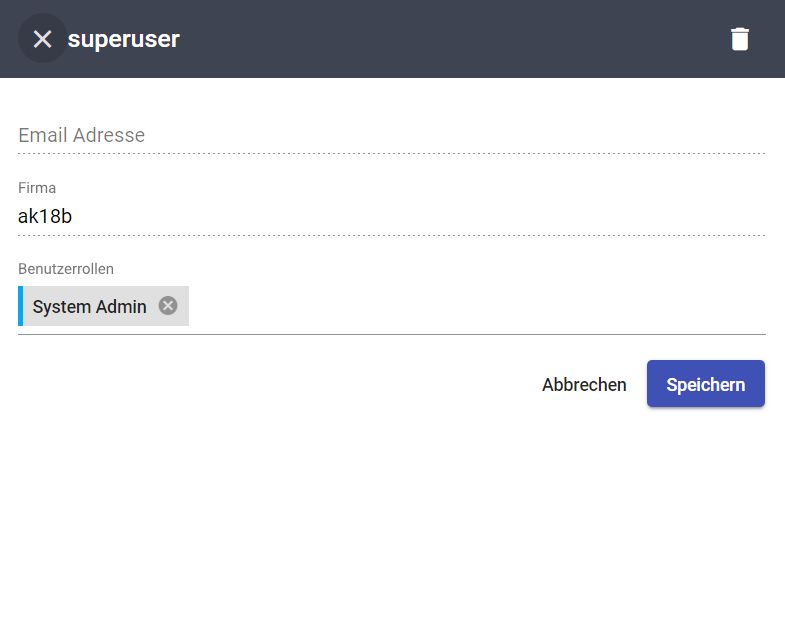
\includegraphics[scale=0.55]{Benutzeredit.png}
	\end{minipage}
	\hfill
	\begin{minipage}{0.4\linewidth}
	\begin{enumerate}[3]
		\item Ändern Sie die Felder
		\item Klicken Sie auf Speichern
	\end{enumerate}
	\end{minipage}\\

	\subsection{Eine Firma hinzufügen}
	
	\begin{enumerate}
		\item Klicken Sie auf \glqq{}Firmen\grqq{}
		\item Klicken Sie auf \texttt{+} neben der Suchleiste
		\item Wählen Sie den Firmennamen
		\item Klicken Sie auf Speichern
	\end{enumerate}\\

\end{document}